\section{Design}
\label{sec:design}

\begin{figure}[ht]
\begin{centering}
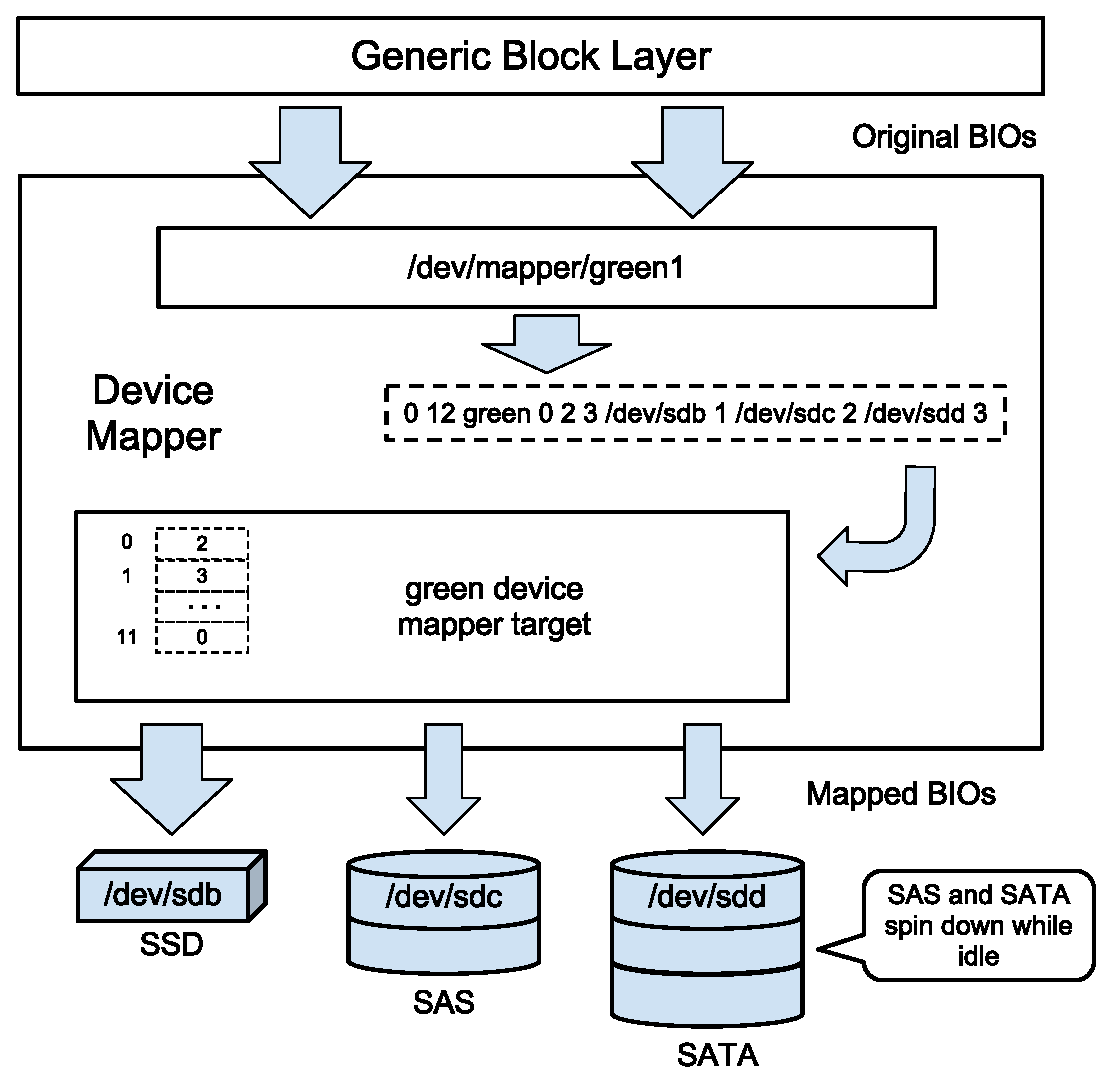
\epsfig{file=figures/dm.eps,width=1.00\linewidth}
\caption{Linux Device Mapper and Green Device Mapper Target.
\texttt{/dev/mapper/green1} is a virtual block device created by the
framework. The two dashed boxes are mapping tables. The first one is
used by the Device Mapper to delegate mapping to target; the second
one is used internally by the green target.}
\label{fig:dm}
\end{centering}
\end{figure}

We implemented our green multi-disk driver as a Linux Device Mapper
target. Linux Device Mapper, as depicted in Figure \ref{fig:dm}, is a
generic framework to map one block device onto another. It works by
processing data passed in from a virtual block device, that it itself
provides, and then passing the resultant data on to another block
device \cite{wiki_dm}. The advantage of Device Mapper is that it can
provide virtual devices to user programs and kernel modules above
block level without exposing underlying devices.  Thanks to this
transparency, the underlying devices can be of different size and type
(can in turn be virtual or physical) and the mapping can be performed
in a different manner. The Device mapper is essentially a middleware
sitting between the Generic Block Layer and block devices. It receives
BIOs, which are kernel structures describing I/O requests, from
Generic Block Layer, then redirect them to other block devices by
modifying the target device and sector offset. 

\begin{figure}[t]
\begin{minipage}[t]{.98\linewidth}
{\footnotesize
  \begin{tabular}{|p{0.9cm}|p{1.0cm}|p{0.9cm}|p{4.5 cm}|}
   \hline
   Offset & Length & Target & Target Parameters \\
   \hline
    0 & 524288 & linear & /dev/sdd 0  \\
    524288 & 1572864 & linear & /dev/sdc 0    \\
   \hline
  \end{tabular}
}
\centerline{(a) A mapping table using the linear target}
\end{minipage}
\begin{minipage}[b]{.98\linewidth}
{\footnotesize
  \begin{tabular}{|p{0.9cm}|p{1.0cm}|p{0.9cm}|p{4.5 cm}|}
   \hline
   Offset & Length & Target & Target Parameters \\
   \hline
   0 & 2097152  & green & 2 8 2 /dev/sdd 65536 /dev/sdc 196608 \\
   \hline
  \end{tabular}
}
\centerline{(b) A mapping table using the green target}
\end{minipage}
\caption{Two mapping tables used in our experiments. One table
corresponds to one virtual device. One entry of the table corresponds
to one range of the virtual device. Offset and Length are in unit of
sectors. Target Parameters are parsed by corresponding target.} 
\label{fig:dmtable}
\end{figure}

The Device Mapper itself does not perform the redirection. It
delegates this operation to Device Mapper targets, which are
registered kernel modules performing certain kinds of mapping. This
delegation is specified in a mapping table, which contains the types
of responsible Device Mapper target for different regions of the
virtual devices created by the framework. Figure \ref{fig:dmtable}
presents two examples. The first table is $524288+1572864$ sectors
large and contains two regions $[0, 524288)$ and $[524288,
524288+1572864)$.  Both of the two regions are handled by the linear
target. The first region maps all I/Os to \texttt{/dev/sdd} starting
from offset 0; the second region maps all I/Os to \texttt{/dev/sdc}
starting from offset 0 as well. The second table corresponds to a
virtual device that is 2097152 sectors large but contains only one
region. The region is handled by the green target.  Device Mapper
targets contain functions to construct/destruct virtual device
regions, map I/O requests, merge adjacent I/O requests, report and
control device status. Parameters of our green target start from three
integers (\texttt{2 8 2} in Figure \ref{fig:dmtable}(b)). The first
one is metadata mode. It tells how to initialize metadata when a
virtual device is created. There are currently three mode. Mode 0
means to create virtual device using metadata previously created on
disk and report failure if no metadata exists; Mode 1 means to use
existing metadata on disk but initialize new metadata if not exists;
Mode 2 means create brand new device and new metadata.  The second
parameter is the size of an extent in unit of sector, which is 8
sectors in the example. The third is the number of underlying physical
disks. The rest are pairs of physical device name and length of the
device in unit of extent. 

\subsection{Design Goals}
The design goal of our green multi-disk Device Mapper target is driven
by the following three guiding principles: 

\begin{enumerate}

\item \textbf{Save energy by allowing disks to spin/power down}.
Energy efficiency is one of the most important features our green
multi-disk target is pursuing. The SSD benefits both I/O performance
and energy efficiency simultaneously. In this study, we are more
concerned about the latter. We have made trade-offs between energy
efficiency and other desirable features such as capacity.

\item \textbf{Use SSD aware data structures and algorithms}. While SSD
provides better I/O performance and energy efficiency, it has its own
constraints including limited erase-write cycles and inefficient
random writes. This principle guides our design to avoid these
constraints and extract the maximum benefit out of an SSD.

\item \textbf{Provide stable and robust storage}. Because our green
target provides customized block mapping and data grouping, it is
critical to always perform correct translation from virtual to
physical blocks. It should not lose mapping information in case of
power failures.

\end{enumerate}

\subsection{Disk Management}

Device Mapper targets maintain mapping of sectors between virtual and
physical disks. The straightforward method is to maintain a
sector-wise mapping table. However, it is prohibitive because its size
is too large to fit in memory. For example, the size of the
sector-wise mapping table of a 1TB disk (512-byte sectors) is as large
as 8GB with 4-byte table entries. Storing the mapping table on disk
(even on SSD) is not an option because it is too slow to incur extra
I/Os. A solution is to divide disks into larger units. Here, we adopt
the term \textit{extent}, which is the unit of disk managed by LVM,
typically 4MB. Then the mapping becomes extent-wise and its size
diminishes to 1MB in the above example. This extent-wise mapping and
migration is encouraged by modern disks, almost all of which support
\texttt{multcount} feature \cite{speed_up}. \texttt{multcount}, short
for multiple sector count, controls how many sectors are fetched from
the disk in a single I/O interrupt. As claimed in \texttt{hdparm}
manual \cite{hdparm}: 

\begin{quotation}
When the \texttt{multcount} feature is enabled, it typically reduces
operating system overhead for disk I/O by 30-50\%. On many systems, it
also provides increased data throughput of anywhere from 5\% to 50\%.
\end{quotation}

In our green target, multiple physical disks are mapped as a single
virtual disk. The physical disks are linearly organized in the order
of energy efficiency, i.e., the most energy-efficient one goes first
and so on. In Figure \ref{fig:dm}, \texttt{/dev/sdb} is the most
energy-efficient one but with smallest capacity, i.e., SSD;
\texttt{/dev/sdc} and \texttt{/dev/sdd} follow decreasingly in energy
efficiency and increasingly in capacity. This makes the addressing of
physical sectors easy. An extent index and an offset within extent
would suffice. We have noticed the case that one I/O request on logically
sequential blocks might be mapped to multiple I/O requests on
physically non-sequential blocks. Namely, the translation is performed
per extent instead of per request. However, extent is of big size, so
it is unlikely that the extent-by-extent translation becomes a
performance bottleneck. Furthermore, the Device Mapper framework
provides an interface to merge adjacent I/O requests, which also
alleviates this problem.

The size of an extent is an important factor because it affects not
only memory consumption but also the granularity of mapping and data
migration. A large size of extent has the following effects: 

\begin{itemize} 

\item \textbf{Smaller mapping table}. As already discussed, the
adoption of extent makes the mapping table becomes extent-wise and
small. 

\item \textbf{More aggressive pre-fetch}. An energy-efficient disk
such as SSD have similar effect as disk cache. When a large extent of
data is moved onto SSD, it can be considered as an aggressive
pre-fetch. 

\item \textbf{Coarse-grained data migration among disks and more
sequential I/O}. Because the major latency of magnetic disks is seek
time, a larger sequential migration does not significantly slow down
the I/O. Moreover, with a large size of migration unit, there are
fewer I/Os because adjacent sectors are processed in batch. This is
beneficial to the lifetime of SSD as well considering its limited
erase-write cycles.

\item \textbf{High overhead}. Since an extent can represent several
sectors, more sectors I/O can be wasted in case of wrong prediction
thus adding overhead to the overall system. 

\end{itemize}

Physical extents are managed using a bitmap. The extents on SSD are
treated specially. Besides being recorded in the bitmap, they are also
linked in two lists, one for free extents and the other for used ones.
This facilitates and speeds up manipulation of the extents on SSD,
which happens frequently.

Different workloads might favor different extent sizes depending on
file sizes, I/O frequency and read-write ratio. Therefore, we make the
extent size a configurable parameter to the green target so that
different trade-offs can be made via configuration. 

%-----------------------------------------------------------------------------

\subsection{Mapping Table}

There are two mapping tables in Figure \ref{fig:dm}. One is actually a
configuration file used by the Device Mapper framework; the other
contains extent-wise mapping information used internally by our green
target. We discuss the second one next.

The straightforward structure of the mapping table is an array of the
size of extent number on all physical disks. Table
\ref{tab:greemtable} shows the structure of the table. The mapping
table is maintained in memory and can be cached, so its lookup is
fast. Besides mapping information, the table also contains other
fields including flags, timestamp of the latest access, and number of
total accesses (possibly distinguished read from write). Flags are
used to record states of extents, which include, for example, 1)
whether the extent is accessed or not recently; 2) whether the extent
is under migration or not; and 3) whether the extent is updated or not
when it is under migration. Timestamp of the latest access and number
of total access are used to predict hot extents.

\begin{table}[t]
{\footnotesize
\centering
\begin{tabular}{r|c|c|c|c|}
\cline{2-5}
\cline{2-5}
  & Physical & & Usage & \\ 
  & Extent ID & Flags & Counter & Timestamp \\
 Virtual Extent Index & 64 bits & 16 bits & 32 bits & 16 bits\\ \cline{2-5} 
 0 & 23 & \dots & \dots & \dots \\
 1 & 9 & \dots & \dots & \dots \\ 
 \vdots & \vdots & \vdots & \vdots & \vdots \\ 
 511 & 234 & \dots & \dots & \dots \\ \cline{2-5}
  \end{tabular}
}
 \caption{Mapping table used by green target. The mapping of virtual
extent $i$ is recored at the $i$-th entry in the table.}
\label{tab:greemtable}

\end{table}

The mapping table needs to be saved onto disks on power off as
metadata. To be fail-safe, it has a replica in every physical disk.
The in-memory version and on-disk version of the mapping table can be
slightly different, since it is not necessary to save online
information such as the timestamp of latest access. To be robust in
case of power failures, the mapping table is flushed onto disk
periodically. To prevent this periodic background job from disturbing
secondary disks' idle periods, this flush saves the table only onto
the cache disk. Tables on other disks are only updated on request or
when the system is being shut down.

%-----------------------------------------------------------------------------

\subsection{Extent Migration}\label{sec:migrate}

The ideal case of our green target is that most I/Os are served using
only the SSD. We try to achieve this by keeping hot extents on the
SSD. However, hot extents are not fixed, they change over time. As an
cold extent becomes hot, we try to migrate it to the SSD. To
accommodate this migration, we have to move an extent on the SSD out if
the SSD was full. Essentially, one migration swaps two extents, one 
extent on one of the secondary disks which becomes hot, and one extent 
on the cache which becomes cold. In total, it involves two reads and 
two writes. To be consistent, incoming I/Os on the migrating extents 
are delayed until the migration is finished.  This elongates latency 
and hurts I/O performance. The following pseudocode describes the 
Read/Write path in using the green target.

To minimize the latency introduced by migration, we divide migration
into two separated operations, promotion and demotion. Promotion moves 
a hot extent from secondary disk onto the SSD, whereas demotion moves 
a cold extent on SSD to secondary disk. We perform demotion operation 
beforehand to ensure that SSD always has free extents available on it,
so that when an promotion operation comes, migration happens straight
away without the need for any other demotions.  In this way, we reduce 
the latency by performing this operation in advance.  Without the division
of demotion and promotion, we need 1) find a cold extent on the SSD,
2) move the cold extent out of the SSD, and 3) bring the hot extent
onto the SSD.  Demotion consists of operation 1 and 2; promotion
consists of operation 3.  

To put demotion ahead, we keep a set of the coldest extents on the
SSD, replicate them on the one of the secondary disks, and mark their
slots on the SSD as available.  When there is a promotion, we
consume one of the available slots and move the hot extent there.  By
consuming one of the available slots, we simply update the mapping of
the old extent to its replica on the secondary disk. In case one of
the extents we maintained as the coldest becomes hot before its slot
is consumed, we move it out of the set and invalidate its replica if
it has been written.

A background thread is used to perform demotion. It makes sure the
size of the set within a range, which is defined by a maximum
threshold and a minimum threshold. Demotion is scheduled when the size
falls under the minimum threshold. This ensures that available extents
can be readily obtained when promotions are needed. Once demotion
kicks start, it keeps demoting more extents until the maximum threshold
is reached. When the range is large, this strategy disturbs secondary
disks less frequently because it batches demoting. Therefore, the
secondary disks are kept idle for longer periods.  It costs space for
the replicas and requires reserved space to make sure there is always
free space. However, the cost is insignificant because they are on
cheap and large secondary disk. 

To find cold extent on SSD, we use the LRU heuristic. Because we can
find cold extents beforehand, we are allowed to use sophisticated LRU
algorithms to obtain good prediction. To predict hot extents, we adopt
a greedy approach and take the extents have just been accessed as hot.
A trade-off between I/O performance and SSD lifetime is possible when
promoting an extent being written. Because SSDs have limited
erase-write cycles, it makes sense to directly map writes to the
secondary disks instead of promoting the extent all at once. If that
extent is read immediately, then we promote it. This is helpful in
case of operations like file copying and file appending, where the
disk is written just once. This does not have a significant impact on
energy efficiency because the secondary disk hosting that extent has
to spin up no matter if we promote it right now or not.  Once it is
up, there is a relative long timeout before it can spin down again
because of the large penalty (latency and short disk lifetime) of disk
spin-down, so no additional spin-up is needed if that extent is read
soon.  Actually, there is research trying to extend SSD lifetime by
using HDD as write cache \cite{hddcache}.  However, this is a
configurable feature that allows users to make informed decisions when
workload knowledge is available. 

\subsection{Data Grouping}

We have studied the data grouping in Wildani et al's work
\cite{Wildani_grouping}, wherein data grouping is workload specific
and is performed offline. A simple heuristic we are going to
experiment is to group data by frequency of access. That is, most
accessed data are all mapped onto the first disk, namely, SSD and so
forth. The reason behind this is that it is likely for data in same
working set to exhibit access frequency at the same level.  Thanks to
our dynamic mapping, we can perform data grouping online as well. Our
migration favors data grouping.  It is likely that extents in a common
working set becomes cold at a same time. It is also likely that they
are demoted onto a single secondary disk instead of being scattered
among multiple disks because our demotions are processed in batch. 

%%%%%%%%%%%%%%%%%%%%%%%%%%%%%%%%%%%%%%%%%%%%%%%%%%%%%%%%%%%%%%%%%%%%%%%%%%%%%%
%% For Emacs:
% Local variables:
% fill-column: 70
% End:
%%%%%%%%%%%%%%%%%%%%%%%%%%%%%%%%%%%%%%%%%%%%%%%%%%%%%%%%%%%%%%%%%%%%%%%%%%%%%%
%% For Vim:
% vim:textwidth=70
%%%%%%%%%%%%%%%%%%%%%%%%%%%%%%%%%%%%%%%%%%%%%%%%%%%%%%%%%%%%%%%%%%%%%%%%%%%%%%
% LocalWords:  
